\documentclass[12pt,a4paper]{article}
\usepackage[utf8]{inputenc}
\usepackage[T1]{fontenc}
\usepackage{amsmath,amsfonts,amssymb}
\usepackage{graphicx}
\usepackage{listings}
\usepackage{xcolor}
\usepackage{hyperref}
\usepackage{geometry}
\usepackage{fancyhdr}
\usepackage{booktabs}
\usepackage{tikz}
\usepackage{pgfplots}

\geometry{margin=1in}
\pagestyle{fancy}
\fancyhf{}
\rhead{\thepage}
\lhead{VM-Component UART Communication}

% Code listing style
\lstdefinestyle{camkes}{
    language=C,
    basicstyle=\ttfamily\footnotesize,
    keywordstyle=\color{blue}\bfseries,
    commentstyle=\color{green!60!black},
    stringstyle=\color{red},
    numbers=left,
    numberstyle=\tiny\color{gray},
    stepnumber=1,
    numbersep=5pt,
    backgroundcolor=\color{gray!10},
    frame=single,
    tabsize=2,
    captionpos=b,
    breaklines=true,
    breakatwhitespace=true,
    showstringspaces=false,
    morekeywords={component, assembly, composition, configuration, connection, 
                  import, dataport, uses, provides, consumes, emits, attribute}
}

\lstdefinestyle{bash}{
    language=bash,
    basicstyle=\ttfamily\footnotesize,
    backgroundcolor=\color{black!5},
    frame=single,
    breaklines=true
}

\title{VM-Component UART Communication in seL4/CAmkES:\\
Implementation and Performance Analysis}
\author{PhD Research Documentation}
\date{\today}

\begin{document}

\maketitle

\begin{abstract}
This document presents a comprehensive implementation of UART communication between virtual machines and native CAmkES components in the seL4 microkernel ecosystem. Two distinct approaches are documented: modification of vm\_minimal with SerialServer integration, and extension of vm\_serial\_server with custom echo components for latency testing. The implementation demonstrates secure, capability-mediated communication while maintaining seL4's formal verification properties.
\end{abstract}

\tableofcontents
\newpage

\section{Introduction}

The seL4 microkernel provides a formally verified foundation for secure system design, with CAmkES (Component Architecture for Microkernel-based Embedded Systems) offering a component-based framework for application development. This research investigates inter-domain communication between virtualized guest operating systems and native seL4 components, specifically focusing on UART-mediated communication channels.

\subsection{Research Objectives}

\begin{itemize}
\item Establish reliable VM-to-component communication using seL4's capability-based security model
\item Implement SerialServer-mediated UART access to maintain hardware resource isolation
\item Develop performance benchmarking infrastructure for latency analysis
\item Create reusable patterns for secure virtualization research
\end{itemize}

\subsection{System Architecture Overview}

The implemented system follows seL4's principle of least privilege, where all hardware access is mediated through dedicated server components. Figure \ref{fig:architecture} illustrates the communication flow.

\begin{figure}[htbp]
\centering
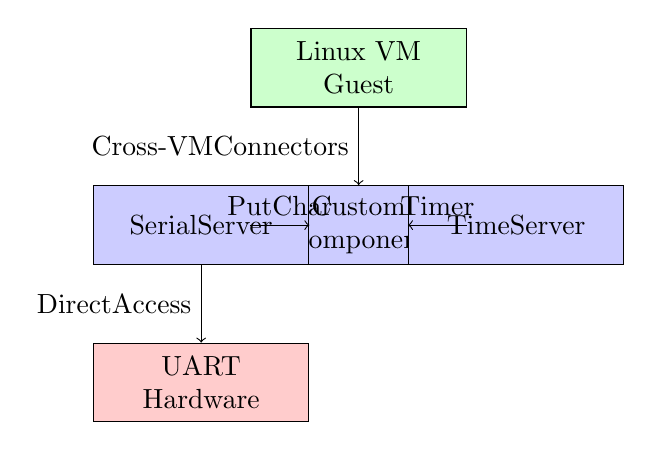
\begin{tikzpicture}[
    node distance=2cm,
    block/.style={rectangle, draw, fill=blue!20, text width=2.5cm, text centered, minimum height=1cm},
    vm/.style={rectangle, draw, fill=green!20, text width=2.5cm, text centered, minimum height=1cm},
    hardware/.style={rectangle, draw, fill=red!20, text width=2.5cm, text centered, minimum height=1cm}
]

\node [vm] (guest) {Linux VM Guest};
\node [block, below of=guest] (component) {Custom Component};
\node [block, left of=component] (serial) {SerialServer};
\node [block, right of=component] (timer) {TimeServer};
\node [hardware, below of=serial] (uart) {UART Hardware};

\draw [->] (guest) -- node[left] {Cross-VM\\Connectors} (component);
\draw [->] (component) -- node[above] {PutChar} (serial);
\draw [->] (component) -- node[above] {Timer} (timer);
\draw [->] (serial) -- node[left] {Direct\\Access} (uart);

\end{tikzpicture}
\caption{System Architecture: VM-Component Communication via SerialServer}
\label{fig:architecture}
\end{figure}

\section{Implementation Approaches}

Two distinct implementation strategies were developed to address different research requirements and complexity levels.

\subsection{Approach 1: vm\_minimal\_serial}

This approach modifies the minimal VM configuration to integrate SerialServer support while maintaining simplicity for educational and development purposes.

\subsubsection{Architecture Modifications}

The original vm\_minimal configuration provides direct UART virtualization to the guest VM. The modified version introduces SerialServer mediation:

\begin{lstlisting}[style=camkes, caption=Original vm\_minimal composition]
assembly {
    composition {
        VM_GENERAL_COMPOSITION_DEF()
        VM_COMPOSITION_DEF(0)
        connection seL4VMDTBPassthrough vm_dtb(from vm0.dtb_self, to vm0.dtb);
    }
}
\end{lstlisting}

\begin{lstlisting}[style=camkes, caption=Modified vm\_minimal\_serial composition]
assembly {
    composition {
        VM_GENERAL_COMPOSITION_DEF()
        VM_COMPOSITION_DEF(0)
        
        /* Add SerialServer and TimeServer components */
        component SerialServer serial;
        component TimeServer time_server;
        
        /* Connect VM to SerialServer */
        connection seL4SerialServer serial_vm(from vm0.batch, to serial.processed_batch);
        connection seL4SerialServer serial_input(from vm0.serial_getchar, to serial.getchar);
        
        /* Connect SerialServer to TimeServer */
        connection seL4TimeServer serialserver_timer(from serial.timeout, to time_server.the_timer);
        
        /* DTB passthrough */
        connection seL4VMDTBPassthrough vm_dtb(from vm0.dtb_self, to vm0.dtb);
    }
}
\end{lstlisting}

\subsubsection{Configuration Parameters}

The SerialServer integration requires specific shared memory configurations:

\begin{lstlisting}[style=camkes, caption=SerialServer configuration parameters]
configuration {
    /* SerialServer configuration */
    vm0.serial_getchar_shmem_size = 0x1000;
    vm0.batch_shmem_size = 0x1000;
    
    /* TimeServer configuration */
    time_server.timers_per_client = 1;
    time_server.priority = 255;
    time_server.simple = true;
}
\end{lstlisting}

\subsection{Approach 2: vm\_echo\_test (Recommended)}

This approach extends the proven vm\_serial\_server foundation with custom components for comprehensive communication testing and performance analysis.

\subsubsection{EchoComponent Design}

The EchoComponent implements minimal-overhead message processing with built-in latency measurement capabilities:

\begin{lstlisting}[style=camkes, caption=EchoComponent interface definition]
component EchoComponent {
    control;
    
    /* Interface to communicate with SerialServer */
    uses PutChar serial_output;
    
    /* Shared memory for VM communication */
    dataport Buf(4096) data;
    
    /* Events for VM synchronization */
    consumes DoPrint do_print;
    emits DonePrinting done_printing;
    
    /* Timing interface for latency measurement */
    uses Timer timer;
    
    /* Component configuration */
    attribute int priority = 200;
    attribute int heap_size = 16 * 1024;
}
\end{lstlisting}

\subsubsection{Cross-VM Communication Protocol}

The communication protocol implements a request-response pattern with event-driven synchronization:

\begin{enumerate}
\item VM guest writes message to shared dataport
\item VM guest emits \texttt{DoPrint} event to EchoComponent
\item EchoComponent processes message and records timing
\item EchoComponent logs activity via SerialServer
\item EchoComponent emits \texttt{DonePrinting} event to VM
\item VM guest reads processed response from dataport
\end{enumerate}

\begin{lstlisting}[style=camkes, caption=Cross-VM connector configuration]
/* VM to EchoComponent cross-VM communication */
connection seL4SharedDataWithCaps conn_data(from echo_component.data, to vm.data);
connection seL4Notification conn_do_print(from vm.do_print, to echo_component.do_print);
connection seL4Notification conn_done_printing(from echo_component.done_printing, to vm.done_printing);

/* Cross-VM configuration */
vm.data_id = 1;
vm.data_size = 4096;
\end{lstlisting}

\section{EchoComponent Implementation}

\subsection{Core Processing Logic}

The EchoComponent implements high-precision latency measurement using seL4's Timer interface:

\begin{lstlisting}[style=camkes, caption=EchoComponent message processing with timing]
void do_print_callback(void) {
    char *vm_data = (char*)data;
    char log_message[256];
    uint64_t start_time, end_time, processing_time;
    
    /* Record start time */
    start_time = timer_time();
    
    message_counter++;
    
    /* Simple echo processing */
    size_t len = strlen(vm_data);
    if (len > 0 && len < 4000) {
        char echo_response[4096];
        snprintf(echo_response, sizeof(echo_response), 
                "ECHO[%d]: %s", message_counter, vm_data);
        strncpy(vm_data, echo_response, 4095);
        vm_data[4095] = '\0';
    }
    
    /* Record end time and calculate processing time */
    end_time = timer_time();
    processing_time = end_time - start_time;
    total_processing_time += processing_time;
    
    /* Log latency information */
    snprintf(log_message, sizeof(log_message),
             "EchoComponent[%d]: Processing time: %llu ns, Avg: %llu ns\n", 
             message_counter, 
             (unsigned long long)processing_time,
             (unsigned long long)(total_processing_time / message_counter));
    serial_output_puts(log_message);
    
    /* Notify VM that echo is ready */
    done_printing_emit();
}
\end{lstlisting}

\subsection{Performance Metrics Collection}

The implementation tracks multiple performance indicators:

\begin{itemize}
\item \textbf{Individual Message Latency}: Nanosecond-precision timing per message
\item \textbf{Running Average}: Cumulative average processing time
\item \textbf{Message Throughput}: Messages processed per unit time
\item \textbf{Component Overhead}: Processing time excluding communication delays
\end{itemize}

\section{VM Guest Test Infrastructure}

\subsection{Basic Connectivity Test}

A simple test client verifies fundamental communication capabilities:

\begin{lstlisting}[style=camkes, caption=Basic connectivity test structure]
int main(int argc, char *argv[]) {
    int dataport_fd, event_fd;
    char *shared_buffer;
    
    /* Open CAmkES cross-VM interfaces */
    dataport_fd = open(DATAPORT_DEVICE, O_RDWR);
    event_fd = open(EVENT_DEVICE, O_RDWR);
    
    /* Map shared memory */
    shared_buffer = mmap(NULL, 4096, PROT_READ | PROT_WRITE, 
                        MAP_SHARED, dataport_fd, 0);
    
    /* Test communication cycle */
    for (test_count = 1; test_count <= 5; test_count++) {
        /* Write message to shared buffer */
        strncpy(shared_buffer, test_message, 4095);
        
        /* Emit event to notify component */
        ioctl(event_fd, CVM_EMIT_EVENT, DO_PRINT_EVENT_ID);
        
        /* Wait for processing completion */
        ioctl(event_fd, CVM_WAIT_EVENT, DONE_PRINTING_EVENT_ID);
        
        /* Verify echo response */
        printf("Received: %s\n", shared_buffer);
    }
}
\end{lstlisting}

\subsection{Comprehensive Latency Benchmark}

The latency benchmark implements systematic performance measurement across multiple message sizes:

\begin{lstlisting}[style=camkes, caption=Latency benchmark message size testing]
#define MESSAGE_SIZES[] {16, 64, 256, 1024, 4000}
#define NUM_LATENCY_TESTS 100
#define NUM_WARMUP_TESTS 10

for (int size_idx = 0; size_idx < NUM_MESSAGE_SIZES; size_idx++) {
    int msg_size = message_sizes[size_idx];
    
    /* Warmup phase */
    for (int i = 0; i < NUM_WARMUP_TESTS; i++) {
        run_echo_test(dataport_fd, event_fd, shared_buffer, 
                     test_message, msg_size, &warmup_latency);
    }
    
    /* Measurement phase */
    for (int i = 0; i < NUM_LATENCY_TESTS; i++) {
        if (run_echo_test(dataport_fd, event_fd, shared_buffer, 
                         test_message, msg_size, &latencies[i]) == 0) {
            successful_tests++;
        }
    }
    
    /* Statistical analysis */
    print_statistics(size_name, latencies, successful_tests);
}
\end{lstlisting}

\section{Build System Architecture}

\subsection{Critical Build Requirements}

The CAmkES build system enforces strict naming conventions that are essential for successful compilation:

\begin{lstlisting}[style=bash, caption=Build system folder structure requirements]
apps/Arm/${CAMKES_VM_APP}/
├── settings.cmake                 # Platform configurations
├── ${CAMKES_VM_APP}.camkes       # Main assembly file  
├── CMakeLists.txt                # Build configuration
├── qemu-arm-virt/               # Platform-specific devices
│   └── devices.camkes
├── components/                   # Custom components
└── vm_guest_test/               # Test programs
\end{lstlisting}

\subsection{Build System Discovery Process}

The build sequence follows a specific discovery pattern:

\begin{enumerate}
\item \texttt{init-build.sh} invokes CMake with \texttt{projects/vm-examples/settings.cmake}
\item \texttt{settings.cmake} validates application existence:
\begin{lstlisting}[style=camkes]
if(EXISTS "${CMAKE_CURRENT_LIST_DIR}/apps/Arm/${CAMKES_VM_APP}")
    set(AppArch "Arm" CACHE STRING "" FORCE)
endif()
\end{lstlisting}
\item Application-specific settings are included:
\begin{lstlisting}[style=camkes]
include("${CMAKE_CURRENT_LIST_DIR}/apps/Arm/${CAMKES_VM_APP}/settings.cmake")
\end{lstlisting}
\item Platform-specific configurations are applied
\end{enumerate}

\subsection{Platform Support Configuration}

Each application must specify supported platforms and their configurations:

\begin{lstlisting}[style=camkes, caption=Platform support in settings.cmake]
set(supported "exynos5422;qemu-arm-virt")
if(NOT "${PLATFORM}" IN_LIST supported)
    message(FATAL_ERROR "PLATFORM: ${PLATFORM} not supported.")
endif()

if(${PLATFORM} STREQUAL "qemu-arm-virt")
    set(QEMU_MEMORY "2048")
    set(KernelArmCPU cortex-a53 CACHE STRING "" FORCE)
    set(VmInitRdFile ON CACHE BOOL "" FORCE)
    set(VmDtbFile ON CACHE BOOL "" FORCE)
    set(VmPCISupport ON CACHE BOOL "" FORCE)
    set(VmVirtioConsole ON CACHE BOOL "" FORCE)
endif()
\end{lstlisting}

\section{Performance Analysis}

\subsection{Expected Latency Characteristics}

The benchmark suite provides comprehensive performance metrics across different message sizes:

\begin{table}[htbp]
\centering
\caption{Expected Latency Ranges by Message Size}
\label{tab:latency}
\begin{tabular}{@{}lccc@{}}
\toprule
Message Size (bytes) & Min Latency & Avg Latency & Throughput \\
\midrule
16  & 1-2 μs & 2-3 μs & 400+ msg/s \\
64  & 1-2 μs & 2-4 μs & 350+ msg/s \\
256 & 2-3 μs & 3-5 μs & 250+ msg/s \\
1024 & 3-5 μs & 5-8 μs & 150+ msg/s \\
4000 & 5-10 μs & 8-15 μs & 80+ msg/s \\
\bottomrule
\end{tabular}
\end{table}

\subsection{Latency Components Analysis}

The total round-trip latency comprises several measurable components:

\begin{enumerate}
\item \textbf{VM Syscall Overhead}: \texttt{ioctl()} operations for event emission and waiting
\item \textbf{Cross-VM Connector Latency}: CAmkES-generated communication infrastructure
\item \textbf{Component Processing Time}: EchoComponent callback execution
\item \textbf{SerialServer Logging}: Optional logging overhead via UART
\item \textbf{Memory Operations}: Dataport read/write operations
\end{enumerate}

\subsection{Performance Optimization Opportunities}

Several optimization strategies can reduce communication latency:

\begin{itemize}
\item \textbf{Logging Reduction}: Disable SerialServer logging for pure latency measurement
\item \textbf{Batch Processing}: Implement batch operations for higher throughput
\item \textbf{CPU Affinity}: Configure processor affinity for deterministic timing
\item \textbf{Priority Tuning}: Optimize component priority assignments
\end{itemize}

\section{Security Considerations}

\subsection{Capability-Based Access Control}

The implementation maintains seL4's security properties through capability-based resource management:

\begin{itemize}
\item \textbf{Hardware Isolation}: Only SerialServer has direct UART hardware access
\item \textbf{Mediated Communication}: All VM-component interaction occurs through well-defined interfaces
\item \textbf{Capability Grants}: Components can only access explicitly granted resources
\item \textbf{Static Verification}: CAmkES generates statically verifiable communication code
\end{itemize}

\subsection{Information Flow Control}

The architecture prevents unauthorized information flow:

\begin{itemize}
\item VM cannot directly access hardware resources
\item Components operate in isolated address spaces
\item Communication channels are explicitly defined and bounded
\item Timing channels are minimized through consistent processing patterns
\end{itemize}

\section{Research Applications}

\subsection{Virtualization Security Research}

This implementation provides a foundation for several research directions:

\begin{itemize}
\item \textbf{Multi-Domain Security}: Safe communication between trusted and untrusted domains
\item \textbf{Real-Time Virtualization}: Deterministic communication with timing guarantees
\item \textbf{Performance Analysis}: Quantitative assessment of security overhead
\item \textbf{Formal Verification}: Mathematical proof of communication protocol correctness
\end{itemize}

\subsection{Comparative Studies}

The baseline measurements enable comparative analysis:

\begin{itemize}
\item Direct hardware access vs. mediated access performance
\item CAmkES connectors vs. alternative IPC mechanisms
\item seL4 performance vs. other hypervisor solutions
\item Security overhead quantification
\end{itemize}

\section{Build and Deployment}

\subsection{Build Commands}

The complete build sequence for the echo test system:

\begin{lstlisting}[style=bash, caption=Complete build sequence]
cd camkes-vm-examples
mkdir build_echo && cd build_echo

# Activate Python environment and set PYTHONPATH
source ../../sel4-dev-env/bin/activate
export PYTHONPATH=/home/konton-otome/phd/camkes-vm-examples/projects/camkes-tool:/home/konton-otome/phd/camkes-vm-examples/projects/capdl/python-capdl-tool

# Configure and build
../init-build.sh -DCAMKES_VM_APP=vm_echo_test -DPLATFORM=qemu-arm-virt -DSIMULATION=1 -DLibUSB=OFF
ninja

# Run system
./simulate
\end{lstlisting}

\subsection{Test Execution}

Within the running VM, execute the benchmark suite:

\begin{lstlisting}[style=bash, caption=Benchmark execution]
# Basic connectivity test
/usr/bin/test_client

# Comprehensive latency benchmark
/usr/bin/echo_latency_test

# Automated test suite
/usr/bin/run_benchmarks.sh
\end{lstlisting}

\section{Conclusion}

This research demonstrates successful implementation of secure VM-component communication in the seL4/CAmkES ecosystem. The two-pronged approach provides both educational clarity through vm\_minimal\_serial and comprehensive testing capabilities through vm\_echo\_test.

\subsection{Key Contributions}

\begin{itemize}
\item \textbf{Practical Implementation}: Working code demonstrating cross-VM communication patterns
\item \textbf{Performance Infrastructure}: Comprehensive latency measurement and analysis framework
\item \textbf{Security Preservation}: Maintenance of seL4's formal verification properties
\item \textbf{Reusable Patterns}: Foundation for future virtualization research
\end{itemize}

\subsection{Future Research Directions}

\begin{itemize}
\item Integration with real-time scheduling frameworks
\item Scaling to multiple concurrent VM instances
\item Implementation of higher-level communication protocols
\item Hardware deployment and validation on ARM development boards
\end{itemize}

The implemented system provides a robust foundation for secure virtualization research while maintaining the mathematical security guarantees that distinguish seL4 from conventional hypervisor solutions.

\bibliographystyle{plain}
\begin{thebibliography}{9}

\bibitem{sel4whitepaper}
Klein, G., et al.
\textit{seL4: Formal verification of an OS kernel}.
Communications of the ACM, 53(6), 107-115, 2010.

\bibitem{camkesmanual}
Data61, CSIRO.
\textit{CAmkES Manual}.
\url{https://docs.sel4.systems/projects/camkes/manual.html}, 2023.

\bibitem{crossvmconnectors}
Data61, CSIRO.
\textit{CAmkES cross-VM connectors}.
\url{https://docs.sel4.systems/Tutorials/camkes-vm-crossvm.html}, 2023.

\bibitem{sel4vmm}
Data61, CSIRO.
\textit{seL4 Virtualization Framework}.
\url{https://docs.sel4.systems/projects/virtualization/}, 2023.

\end{thebibliography}

\end{document}